\documentclass{article}

\textwidth=6.5in
\textheight=8.5in
\voffset=-54pt
\oddsidemargin=0in
\evensidemargin=0in
\setlength{\parskip}{8pt}
\setlength{\parindent}{0pt}

\usepackage{amsmath, amssymb}
\usepackage{ifthen}

\usepackage[inline]{enumitem}
\setlist{topsep=0pt, parsep=8pt}

\usepackage[rgb,table]{xcolor}\convertcolorsUfalse
\usepackage{graphicx}

% change hyperref options
\PassOptionsToPackage{hyphens}{url}
\usepackage[bookmarks,colorlinks,linkcolor=black,citecolor=blue,pdfstartview=FitH,urlcolor=blue]{hyperref}
\hypersetup{pdfpagemode=UseNone}
\usepackage{bookmark}

\usepackage{graphicx}
\usepackage{multicol}
\usepackage{framed}
\usepackage{array}

\usepackage{icomma}

\usepackage{pifont}

\usepackage{soul}

\usepackage{pgfplots}
\pgfplotsset{compat=1.18}  
\pgfplotscreateplotcyclelist{mycolor}{black, blue, red, green!70!black, magenta, purple, cyan, orange }  
\pgfplotsset{
  disabledatascaling,
  cycle list=tikzcolor, 
  axis lines=middle,
  every axis plot/.style={no marks, thick},
  every axis/.style={
    enlarge x limits=false,
    enlarge y limits=auto,
    xlabel style={at={(current axis.right of origin)},anchor=west},
    ylabel style={at={(current axis.above origin)},anchor=south},
    % extra x and y ticks for asymptotes
    extra x tick style={grid=major, grid style={dashed,black}},
    extra y tick style={grid=major, grid style={dashed,black}},
    /pgf/number format/1000 sep={},
  },    
  tick label style = {font=\footnotesize, fill=\currentbgcolor, inner sep=0pt},    
  xticklabel shift=1pt,    
  scaled ticks=false,
  scaled y ticks=false,
  unbounded coords=jump,
  samples=101,
  minor tick length=0,
  scatter/classes={
    open={mark=*,draw=black,fill=white, mark size=2, thin},
    closed={mark=*,draw=black,fill=black, mark size=2, thin}
  },
  width=3in,
}
\pgfplotsset{open/.style={only marks, mark=*, fill=white, thin, mark size=2}}
\pgfplotsset{closed/.style={only marks, mark=*, draw=black, fill=black,
    thin, mark size=2}}
\pgfplotsset{labeled/.style={nodes near coords, only marks, mark=*, draw=black, fill=black, thin, mark size=2, point meta=explicit symbolic}}

\usepackage{tikz}
\usetikzlibrary{
  matrix,%
  % enables the snake paths
  decorations.pathmorphing,%
  % enables bigger arrows
  decorations.markings,%
  decorations.pathreplacing,%
  decorations.text,%
  calc,%
  patterns,%
  shapes.geometric,%
  arrows,
  decorations.shapes,
  positioning,
  plotmarks,
  intersections
}
\tikzset{>=latex} % sets default arrow type in tikz
\tikzset{font=\normalsize}
\tikzset{mark size=1.5pt, mark options=thin}
\tikzset{pin distance=4pt,
  every pin edge/.style={<-, thin, shorten <= -2pt}}

\interfootnotelinepenalty=10000
\renewcommand{\thefootnote}{(\arabic{footnote})}

\usepackage{multirow, bigdelim}

% change to \usepackage[sols]{handout} to see solutions
\usepackage[]{handout}

\providecommand{\check}{}
\renewcommand{\check}{\ifmmode{\text{ \ding{51} }}\else{\ding{51} }\fi}

\newcommand\iscurrentenumi[1]{%
  \ifthenelse{\equal{#1}{\theenumi}}{}{#1}}
\setenumerate[1]{ref=\#\arabic*}
\setenumerate[2]{ref=\protect\iscurrentenumi{\theenumi}(\alph*)}
\newcommand\enumiiprefix[2]{%
  \ifthenelse{{\equal{#1}{\theenumi}}\AND{\equal{#2}{(\alph{enumii})}}}{}{}%
  \ifthenelse{{\equal{#1}{\theenumi}}\AND{\NOT{\equal{#2}{(\alph{enumii})}}}}{#2}{}%
  \ifthenelse{\equal{#1}{\theenumi}}{}{#1#2}%
}
\setenumerate[3]{ref=\protect\enumiiprefix{\theenumi}{(\alph{enumii})}\roman*}

\newlength{\tipmargin}
\makeatletter

\newdimen\SOUL@dimen %new
\def\SOUL@ulunderline#1{{%
    \setbox\z@\hbox{#1}%
    % \dimen@=\wd\z@
    \SOUL@dimen=\wd\z@ %new
    \dimen@i=\SOUL@uloverlap
    \advance\SOUL@dimen2\dimen@i %\dimen@ exchanged too
    \rlap{%
      \null
      \kern-\dimen@i
      % \SOUL@ulcolor{\SOUL@ulleaders\hskip\dimen@}%
      \SOUL@ulcolor{\SOUL@ulleaders\hskip\SOUL@dimen}% new
    }%
    \unhcopy\z@
  }}

\renewenvironment{framed}{
  \setlength{\tipmargin}{\textwidth-\linewidth}
  \advance\@totalleftmargin-\tipmargin
  \def\FrameCommand{\hspace{\tipmargin}\fbox}%
  \advance\linewidth\tipmargin
  \MakeFramed {\advance\hsize-\width \FrameRestore}%
}
{\endMakeFramed}

\makeatother

\definecolor{purple}{rgb}{0.5,0,1.0}

\definecolor{magenta}{rgb}{1, 0, 0.5}

\usepackage{fancyhdr}
\lhead{\textcolor{white}{This content is protected and may not be shared, uploaded, or distributed.}}
\rhead{}
\rfoot{\vspace*{\fill}\footnotesize\textcopyright{} \emph{Harvard Math Ma}}
\renewcommand{\headrulewidth}{0pt}
\pagestyle{fancy}
\begin{document}

\htitle{24. Applications of Exponentials}

\begin{problemonly}
  \begin{framed}

You should be able to:
    \begin{itemize}[topsep=0pt,partopsep=0pt,parsep=8pt,itemsep=0pt]
    \item Model constant percent change over different intervals (like ``decreases by 30\% every 12 hours'' or ``triples every 4 days''), including compound interest.

    \item Explain what \emph{half-life} means, and model phenomena that have a half-life. 

    \item Reason about how an exponential function grows or decays over different time intervals. (For example, if a quantity grows by 10\% every year, will it grow by exactly 20\%, more than 20\%, or less than 20\% in 2 years?)

    \end{itemize}
  \end{framed}
\end{problemonly}

\begin{enumerate}
\item 

  \note{I will talk about both the fact that exponentials have a constant percent change and that they get multiplied by the same factor every day/month/year/whatever the unit of input is.}

  \begin{problem}[\vfill]
    Last time, we talked about exponential functions; what was special
    about them?
  \end{problem}

  \begin{solution}
    Exponential functions exhibit a constant percent change, which is
    the same as saying that the output is multiplied by the same factor
    every day/month/year/unit of input.
  \end{solution}

\item  

  \emph{Warm up.}

  \begin{enumerate}
  \item
    \begin{problem}[\vfill]
      If the population of a country after $t$ years is $5 (1.07)^t$ million people, by what percent is the population growing each year?
    \end{problem}

    \begin{solution}
      Each year, the population is multiplied by $1.07$, which corresponds to a 
      percent change of $1.07-1 = 0.07$, or $7\%$.
    \end{solution}

  \item \label{warmup-exponential-function-to-percent-change}

    \note{In questions like this, it's okay for students to leave the answer as a decimal rather than a percent. (That is, it's fine for them to write $b - 1$ as opposed to $100 (b - 1)$\%.)}

    \begin{problem}[\vfill\newpage]
      Generalize: if the population after $t$ years is instead $f(t) = C \cdot b^t$, what's the percent change per year? 
    \end{problem}

    \begin{solution}
      Each year, we multiply by $b$, so the percent change
      would be $b-1$, which we could multiply by $100$ to convert to a percent, $100(1-b) \%$.
    \end{solution}

  \end{enumerate}

\item  (\href{https://people.math.harvard.edu/~jjchen/mathma/docs/homework/PS22.html}{Problem Set 22}, {{\#3}})

  Each week, Lallemand starts with 0.00005 pounds of yeast; the amount of yeast doubles every 4 hours.

  \begin{enumerate}
  \item

    \note{Students did this in homework, but it was guided, so they might not have really understood the strategy. I want to recap the strategy here of making a table (and how we pick what times to put in the table).}

    \begin{problem}[\vfill]
      Write a formula that gives the number of pounds of yeast $t$ hours after the start of the week. 
    \end{problem}
    
    \begin{solution}
      See \href{https://people.math.harvard.edu/~jjchen/mathma/docs/homework/PS22.html}{Problem Set 22}, {{\#3}}.
    \end{solution}

  \item

    \note{This part wasn't on the homework. We'll just convert the table to days: knowing what happens every 4 hours is the same as knowing what happens every $\frac{1}{6}$ day.}

    \begin{problem}[\vfill]
      Write a formula that gives the number of pounds of yeast $s$ days
      after the start of the week.
    \end{problem}

    \begin{solution}
      We can adjust our table from \href{https://people.math.harvard.edu/~jjchen/mathma/docs/homework/PS22.html}{Problem Set 22}, {{\#3}} so that time is in days:
      \begin{center}
        \begin{tabular}{c | c}
          $s$ & pounds of yeast $s$ days after the start of the week \\
          \hline
          0 & $0.00005$ \\
          $\dfrac{1}{6}$ & $0.00005 (2) = 0.001$ \\
          $\dfrac{2}{6}$ & $0.00005 (2)^2 = 0.002$ \\
          $\dfrac{3}{6}$ & $0.00005 (2)^3 = 0.004$ 
        \end{tabular}
      \end{center}
      So, there are $\boxed{0.00005 (2)^{6s}}$ pounds of yeast after $s$ days. 
    \end{solution}

  \end{enumerate}

\item  \label{compound-interest} \textbf{Finance (compound interest).} 
  \begin{enumerate}

  \item \label{marius-compound-annually}

    \begin{problem}[\nstretch{0.75}]
      Marius decides to open a bank account with an opening deposit of \$1000. Suppose that the account earns a nominal annual interest rate of 6\%, compounded annually.\footnote{The word ``nominal'' means ``in name only''. For economists, there are two uses of the phrase ``nominal interest rate''; one is trying to account for the effects of inflation. We're using it in the other sense, which will be easier to understand after you do \ref{marius-compound-quarterly}.} Assuming Marius completely ignores the account after he opens it (so he doesn't make any deposits or withdrawals), how much money does the account have $t$ years after Marius opens it? 
    \end{problem}

    \begin{solution}
      At the end of each year, he earns 6\% interest, which has the effect of multiplying his balance by $1 + 0.06$. Therefore, after $t$ years, Marius has $1000 (1 + 0.06)^t$. 
    \end{solution}

  \item \label{marius-compound-quarterly}

    \note{I will explain the meaning of quarterly compounding, and then I'll have students try this by making a table.}

    \begin{problem}[\vfill]
      Suppose that Marius had instead deposited his money in a bank that
      offered a 6\% nominal annual interest rate, compounded
      \emph{quarterly} (4 times a year).  This means that, each quarter, 
      the account earns \fitb{0.5in}{$\tfrac{1}{4}\cdot 6$}\% interest.  How much money would
      the account have after $t$ years?
    \end{problem}

    \begin{solution}
      Quarterly compounding with a nominal annual interest rate of 6\% means that, each quarter, the account earns $\frac{1}{4} \cdot 6$\% interest. So, each quarter, the value of the account is multiplied by $1 + \frac{0.06}{4}$. After $t$ years, $4t$ quarters have passed, so the account will have $\boxed{1000 \left( 1 + \frac{0.06}{4} \right)^{4t}}$ dollars.

      Notice that, after one year, Marius has $1000 \left(1 + \frac{0.06}{4} \right)^4 = 1061.36$ dollars. So, he's earned slightly more than 6\% interest over the course of the year. Saying that the ``nominal annual interest rate'' is 6\% distinguishes this rate from the actual interest he earns over the course of the year.

      Again, the money would not really be a continuous function of time, since the interest would only be credited at the end of each quarter.
    \end{solution}

    \note{There are two ways to do this, and I will probably talk about both. One is to use the percent change formula to calculate, say, the percent change from $t = 0$ to $t = 4$. Another one is to recognize that $1000 \left( 1 + \frac{0.06}{4} \right)^{4t}$ is $C \cdot b^t$ with $b = \left( 1 + \frac{0.06}{4} \right)^4$ and then use \ref{warmup-exponential-function-to-percent-change}.

      Once they've done this problem, we can explain the term ``nominal annual interest rate'' better: in this example, Marius earns slightly more than 6\% on his investment over the course of the year because of compounding.}

    \begin{problem}[\stretch{0.75}]
      In this account, what is the percent increase in money per year? (This is called the \textit{annual percentage yield} of the account.)
    \end{problem}

    \begin{solution}
      $\left( 1 + \frac{0.06}{4} \right)^4 - 1$; using a calculator, this
      is 0.06136, or $6.136$\%. 
    \end{solution}

    \note{We can calculate that the APY is higher than the nominal annual interest rate, but I also really want students to have some intuition for why this is. I've found it helpful to be very concrete: with yearly compounding, you earn \$60 of interest in the first year. With quarterly compounding, you earn \$15 the first quarter, but then you start earning interest on that \$15, so you will end the year having earned more than \$60 of interest.} 

  \item

    \note{When $n = 365$, the APY is 6.183\%. So, although it's greater than what we'd get with quarterly compounding, there isn't a huge difference. (In Mb, students will look at continuous compounding.)}

    \begin{problem}[\vfill\newpage]
      What if Marius had used a bank that offered 365 compounding periods a year? How much money would the account have after $t$ years, and what would the annual percentage yield be?
    \end{problem}

    \begin{solution}
      After $t$ years, he would have $\boxed{1000 \left(1 + \frac{0.06}{365} \right)^{365t}}$ dollars.

      The annual percentage yield (as a decimal) is then $\left( 1 + \frac{0.06}{365} \right)^365 - 1 \approx 0.06183$, or 6.138\%.
    \end{solution}

  \end{enumerate}

\item  \label{exp-radium-226} \textbf{Chemistry (radioactive decay).} The half-life of the radioactive isotope radium-226 is approximately 1600 years. This means that, every 1600 years, the amount of radium-226 \probonly{$\vphantom{\dfrac{1}{1}}$}\fitb{1.75in}{gets multiplied by $\frac{1}{2}$}.

  \begin{enumerate}
  \item
    \begin{problem}[\vfill]
      Suppose you have a sample of radium-226 whose size in mg is currently $S_0$. Write a formula for the amount of radium-226 that remains in the sample $t$ centuries from now.
    \end{problem}

    \begin{solution}
      $S(t) = S_0 \left( \frac{1}{2} \right)^{t / 16}$. 
    \end{solution}

    \note{Plugging in $16$ for $t$ is a great way to check.}

    \begin{problem}[\stretch{0.25}]
      \check What's a quick way to check that your answer is reasonable?
    \end{problem}

    \begin{solution}
      We can plug in $t=16$. $S(16) = S_0\left(\frac{1}{2}\right)^{16/16} = \frac{1}{2}S_0$.
    \end{solution}

  \item

    \begin{problem}[\vfill]
      Sketch a graph of the amount of radium-226 in the sample as a function of time.
    \end{problem}

    \begin{solution}
      We know that the $y$-intercept is at $(0, S_0)$, and we also know that
      the graph passes through the point $(16, \frac{1}{2}S_0)$. The amount of radium-226
      decays exponentially, so there is a horizontal asymptote at $y=0$.
    
      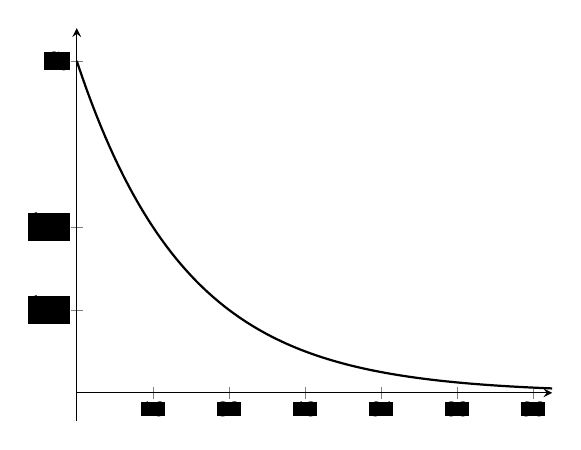
\begin{tikzpicture}
        \begin{axis}[xtick distance=16, ytick={125, 250, 500},
          yticklabels={$\frac{1}{4}S_0$, $\frac{1}{2}S_0$, $S_0$}]
          \addplot[domain=0:100] {500*(0.5)^(x/16)};
        \end{axis}
      \end{tikzpicture}
    \end{solution}

  \item

    \begin{problem}[\stretch{0.35}]
      Every exponential function can be written in the form $C \cdot b^t$; what are $C$ and $b$ for the exponential function you wrote down in (a)?
    \end{problem}

    \begin{solution}
      Let's use exponent rules to rewrite our formula.
      $S(t) = S_0\left(\frac{1}{2}\right)^{t/16} = 
      S_0 \left[\left(\frac{1}{2}\right)^{1/16}\right]^t$.
      From this, we can see that $C=S_0$ and $b = \left(\frac{1}{2}\right)^{1/16}$.
    \end{solution}

  \item
    \begin{problem}[\nstretch{0.35}]
      Suppose you have a sample of radium-226. By what percent does the amount of radium-226 in the sample change per century?
    \end{problem}

    \begin{solution}
      Every 100 years, the amount of radium-226 is multiplied by 
      $\left(\frac{1}{2}\right)^{1/16}$, which is a percent change
       of $\left(\frac{1}{2}\right)^{1/16}-1$, approximately $-0.042$ or $-4.2\%$.
    \end{solution}

  \item
    \begin{problem}[\stretch{0.75}]
      How many years would it take a 100 mg sample of radium-226 to decay
      to 25 mg? 
    \end{problem}

    \begin{solution}
      This would take two half-lives, or 3200 years.
    \end{solution}

  \item \label{exp-radium-226-estimate}

    \note{The point here is that we can't calculate this exactly, although we can tell that it takes between 3 and 4 half-lives, so between 4800 and 6400 years.}

    \begin{problem}[\stretch{0.75}]
      How many years would it take a 100 mg sample of radium-226 to decay to 10 mg? 
    \end{problem}

    \begin{solution}
      This would take between 3 and 4 half-lives, so between 4800 and 6400 years, but we
      haven't yet learned how to find the exact number of years. We would need to
      solve the equation $100\left(\frac{1}{2}\right)^{t/16} = 10$.
    \end{solution}

  \end{enumerate}

\item  \textbf{Sociology.} The population in a certain area of the country is increasing. In 1990 the population was 100,000; by 2010, it was 200,000.

  \begin{enumerate}

  \item
    \begin{problem}[\vfill]
      If the population increased linearly between 1990 and 2010, was the population in 2000 equal to 150,000, greater than 150,000, or less than 150,000? Explain your reasoning with a picture.
    \end{problem}

    \begin{solution}
      The average rate of change of the population between 1990 and 2010 was 
      \[\frac{200,000\text{ people} - 100,000\text{ people}}{10 \text{ years}} = 5,000 
      \text{ people/year}.\]
      If the population was increasing linearly, then the population in the year 2000
      would have been exactly
      \[100,000\text{ people} + (5,000\text{ people/year})(10\text{ years}) = 
      150,000\text{ people}.\]
    \end{solution}

  \item
    Suppose instead that the population increased exponentially between 1990 and 2020.

    \begin{enumerate}
    \item 
      \begin{problem}[\vfill]
        Under this assumption, was the population in 2000 equal to 150,000, greater than 150,000, or less than 150,000? Explain your reasoning with a picture.
      \end{problem}

      \begin{solution}
        Let's compare the graph of a linear function passing through the points
        $(1990, 100,000)$ and $(2010, 200,000)$ with an exponential function passing
        through the same points.
        \begin{center}
          \begin{tikzpicture}
            \begin{axis}[yticklabel style={/pgf/number format/fixed}, disabledatascaling=false, height=2in, xmax=2010.1]
              \addplot+[domain=1990:2010] [ultra thick, red] {5000*(x-1990)+100000}; %
              \addplot+[domain=1990:2010] [ultra thick, blue] {100000*(e^(.69*(x-1990)/20)}; %
            \end{axis}
          \end{tikzpicture}
        \end{center}
        We see that the exponential function is below the linear function. This means that if
        the population grew exponentially, there would have been fewer than 150,000 people
        in 2000.
      \end{solution}

    \item
      \begin{problem}[\nstretch{0.25}]
        Under this assumption, was the population in 2020 equal to 250,000, greater than 250,000, or less than 250,000? Explain.
      \end{problem}

      \begin{solution}
        A population of $250,000$ would correspond to linear growth from 2010 to 2020.
        After 2010, the exponential function overtakes the linear function,
        so under an assumption of exponential growth, the population in 2020 would have been
        greater than 250,000.
        \begin{center}
          \begin{tikzpicture}
            \begin{axis}[yticklabel style={/pgf/number format/fixed}, disabledatascaling=false, height=2in, xmax=2020.1]
              \addplot+[domain=1990:2020] [ultra thick, red] {5000*(x-1990)+100000}; %
              \addplot+[domain=1990:2020] [ultra thick, blue] {100000*(e^(.69*(x-1990)/20)}; %
            \end{axis}
          \end{tikzpicture}
        \end{center}
      \end{solution}
    \end{enumerate}

  \end{enumerate}

\item 

  \note{This is practice applying our knowledge about transforming functions, as well as algebra practice.}

  In each part, you're given a function. Do the following two things:
  \begin{itemize}
  \item Sketch its graph. Label all intercepts and asymptotes. 
  \item Decide whether the function is exponential. If so, it can be written as $f(t) = C \cdot b^t$; identify $C$ and $b$. 
  \end{itemize}

  \begin{enumerate}
  \item
    \begin{problem}[\vfill]
      $f(t) = 4 \cdot 2^{-t/4}$
    \end{problem}

    \begin{solution}
      This is an exponential function, $C=4, b=2^{-1/4}$. Since 
      $2^{-1/4} = \frac{1}{\sqrt[4]{2}}$ is less than 1, this is an exponential decay
      function. The $y$-intercept is at $y=4$ and the horizontal asymptote is $y=0$.
      
      \begin{tikzpicture}
        \begin{axis}[ytick={4}, xtick=\empty, height=2in, axis on top]
          \addplot[domain=-10:10] {4*2^(-x/4)};
        \end{axis}
      \end{tikzpicture}
    \end{solution}

  \item
    \begin{problem}[\vfill]
      $f(t) = \left( \dfrac{1}{3} \right)^{t + 1} - 3$
    \end{problem}

    \begin{solution}
      This function is not exponential because it cannot be written as $f(t)=C\cdot b^t$.
      Its graph is the graph of $y=(\frac{1}{3})^t$, which is an exponential decay
      function, but shifted to the right
      by 1 unit and down 3 units. The $y$-intercept is at $y=-\frac{8}{3}$ and 
      the horizontal asymptote is $y=-3$.

      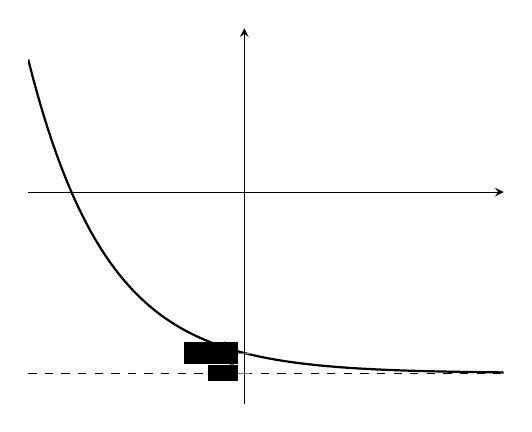
\begin{tikzpicture}
        \begin{axis}[ytick={-8/3}, yticklabels={$-8/3$}, xtick=\empty, extra y ticks={-3},
        height=2.5in, axis on top]
          \addplot[domain=-2.5:3] {(1/3)^(x+1) - 3};
        \end{axis}
      \end{tikzpicture}
    \end{solution}

  \item

    \note{Unlike the previous two, this one really needs to be simplified before we can graph it.}

    \begin{problem}[\vfill]
      $f(t) = 5^{t - 2} \cdot 6^{-t/2}$
    \end{problem}

    \begin{solution}
      This is an exponential function. We can rewrite it as
      \begin{align*} 
        f(t) &= 5^{t-2}\cdot 6^{-t/2} \\
        &= 5^t \cdot 5^{-2} \cdot (6^{-1/2})^t \\
        &= 5^{-2} \cdot (5 \cdot 6^{-1/2})^t
      \end{align*}
      so $C=5^{-2}$, and $b = 5\cdot 6^{-1/2}$. Since 
      $b=5\cdot 6^{-1/2}=\frac{5}{\sqrt{6}}$ is greater than 1, this is an exponential
      growth function. The $y$-intercept is at $y=\frac{1}{25}$ and the horizontal
      asymptote is at $y=0$.

      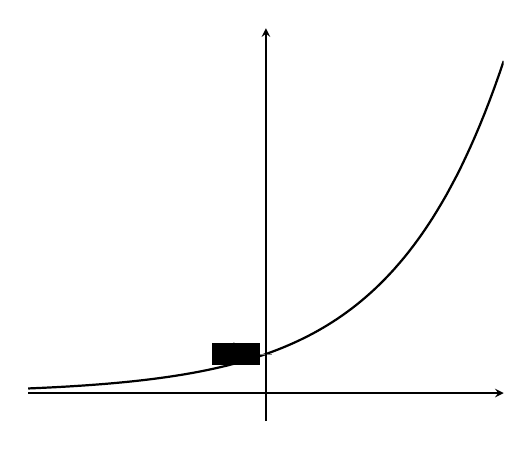
\begin{tikzpicture}
        \begin{axis}[ytick={1/25}, yticklabels={$1/25$}, xtick=\empty, axis on top]
          \addplot[domain=-3:3] {5^(x-2) * 6^(-x/2)};
        \end{axis}
      \end{tikzpicture}
    \end{solution}

  \end{enumerate}

\end{enumerate}
\end{document}
